\documentclass[a4paper,12pt, oneside]{book}

% \usepackage{fullpage}
\usepackage[italian]{babel}
\usepackage[utf8]{inputenc}
\usepackage{amssymb}
\usepackage{amsthm}
\usepackage{graphics}
\usepackage{amsfonts}
\usepackage{listings}
\usepackage{amsmath}
\usepackage{amstext}
\usepackage{engrec}
\usepackage{rotating}
\usepackage{verbatim}
\usepackage[safe,extra]{tipa}
%\usepackage{showkeys}
\usepackage{multirow}
\usepackage{hyperref}
\usepackage{microtype}
\usepackage{fontspec}
\usepackage{enumerate}
\usepackage{physics}
\usepackage{braket}
\usepackage{marginnote}
\usepackage{pgfplots}
\usepackage{cancel}
\usepackage{polynom}
\usepackage{booktabs}
\usepackage{enumitem}
\usepackage{framed}
\usepackage{pdfpages}
\usepackage{pgfplots}
\usepackage{algorithm}
% \usepackage{algpseudocode}
\usepackage[cache=false]{minted}
\usepackage{mathtools}
\usepackage[noend]{algpseudocode}

\usepackage{tikz}\usetikzlibrary{er}\tikzset{multi  attribute /.style={attribute
    ,double  distance =1.5pt}}\tikzset{derived  attribute /.style={attribute
    ,dashed}}\tikzset{total /.style={double  distance =1.5pt}}\tikzset{every
  entity /.style={draw=orange , fill=orange!20}}\tikzset{every  attribute
  /.style={draw=MediumPurple1, fill=MediumPurple1!20}}\tikzset{every
  relationship /.style={draw=Chartreuse2,
    fill=Chartreuse2!20}}\newcommand{\key}[1]{\underline{#1}}
  \usetikzlibrary{arrows.meta}
  \usetikzlibrary{decorations.markings}
  \usetikzlibrary{arrows,shapes,backgrounds,petri}
\tikzset{
  place/.style={
        circle,
        thick,
        draw=black,
        minimum size=6mm,
    },
  transition/.style={
    rectangle,
    thick,
    fill=black,
    minimum width=8mm,
    inner ysep=2pt
  },
  transitionv/.style={
    rectangle,
    thick,
    fill=black,
    minimum height=8mm,
    inner xsep=2pt
    }
  } 
\usetikzlibrary{automata,positioning,chains,fit,shapes}
\usepackage{fancyhdr}
\pagestyle{fancy}
\fancyhead[LE,RO]{\slshape \rightmark}
\fancyhead[LO,RE]{\slshape \leftmark}
\fancyfoot[C]{\thepage}
\usepackage[usenames,dvipsnames]{pstricks}
\usepackage{epsfig}
\usepackage{pst-grad} % For gradients
\usepackage{pst-plot} % For axes
\usepackage[space]{grffile} % For spaces in paths
\usepackage{etoolbox} % For spaces in paths
\makeatletter % For spaces in paths
\patchcmd\Gread@eps{\@inputcheck#1 }{\@inputcheck"#1"\relax}{}{}
\makeatother

\title{Bioinformatica}
\author{UniShare\\\\Davide Cozzi\\\href{https://t.me/dlcgold}{@dlcgold}}
\date{}

\pgfplotsset{compat=1.13}
\begin{document}
\maketitle

\definecolor{shadecolor}{gray}{0.80}
\setlist{leftmargin = 2cm}
\newtheorem{teorema}{Teorema}
\newtheorem{definizione}{Definizione}
\newtheorem{esempio}{Esempio}
\newtheorem{corollario}{Corollario}
\newtheorem{lemma}{Lemma}
\newtheorem{osservazione}{Osservazione}
\newtheorem{nota}{Nota}
\newtheorem{esercizio}{Esercizio}
\algdef{SE}[DOWHILE]{Do}{doWhile}{\algorithmicdo}[1]{\algorithmicwhile\ #1}
\tableofcontents
\renewcommand{\chaptermark}[1]{%
  \markboth{\chaptername
    \ \thechapter.\ #1}{}}
\renewcommand{\sectionmark}[1]{\markright{\thesection.\ #1}}
\newcommand{\floor}[1]{\lfloor #1 \rfloor}
\newcommand{\MYhref}[3][blue]{\href{#2}{\color{#1}{#3}}}%
\chapter{Introduzione}
\textbf{Questi appunti sono presi a lezione. Per quanto sia stata fatta
  una revisione è altamente probabile (praticamente certo) che possano
  contenere errori, sia di stampa che di vero e proprio contenuto. Per
  eventuali proposte di correzione effettuare una pull request. Link: }
\url{https://github.com/dlcgold/Appunti}.\\
\chapter{Introduzione alla bioinformatica}
La genomica ha dimostrato negli ultimi anni ha dimostrato una capacità
incredibile di produrre dati e questo ha portato alla nascita del
bioinformatico, che diventa un esperto della gestione di questi dati sia dal
punto di vista algoritmico che dal punto vista sistemistico.\\
A partire dal 2000/2001 ma sopratutto poco prima del 2010 si ha una crescita dei
\textbf{dati genomici} non indifferente. I dati genomici sono quelli provenienti
dal sequenziamento del DNA. Negli ultimi anni questa crescita ha superato la
curva della \textbf{legge di Moore} quindi la crescita in termini di hardware
(che si stima migliorare ogni 18 mesi) non riesce più a soddisfare la stima di
richiesta di hardware necessario per il sequenziamento. Questa stima di
sequenziamento è basata su Illumina, che produce le più diffuse macchine fisiche
per il sequenziamento. Case farmaceutiche e laboratori che studiano il
sequenziamento hanno almeno una macchina Illumina. La quantità di dati ha
raggiunto i livelli dei petabyte e quindi ci si aspetta (e in parte già è così)
che l'hardware non sia più in grado di elaborare tali dati.\\
La bioinformatica riceve quindi questa tipologia di dati. La bioinformatica è
cruciale nell'ambito della ricerca in biologia molecolare (riguardante
prettamente DNA), dove sempre più si ha necessità dell'appoggio
dell'informatica, avendo a che fare con dati, nel dettaglio grandi dati.\\
Un altro aspetto è quello legato alle nanotecnologie e alla così detta
\textbf{DNA-based computation}. Un esempio è legato al fatto che ormai si è in
grado di manipolare il DNA al punto di essere in grado di assemblarlo in
laboratorio, tramite un meccanismo a \textit{tiling (tasselli)}, dove il tiling
tendenzialmente è una figura regolare (triangolare, rettangolare, esagonale,
etc$\ldots$) con cui si compone del materiale biologico. Si riescono a fare
letteralmente figure con il DNA (anche stelle, smile etc$\ldots$) ma, sopratutto
di questi tempi, vaccini, che sono appunto manipolazione genetica di DNA o
RNA. \textbf{Questa parte non è trattata nel corso}.
\section{Breve introduzione biologica}
Nel corso tratteremo prevalentemente sequenze di DNA. All'interno della cellula
si hanno i \textbf{cromosomi} e un \textbf{genoma} altro non è che la collezione
di cromosomi all'interno di un individuo. Il singolo cromosoma è rappresentato
da filamenti di DNA ``attorcigliati''. Il cromosoma sostanzialmente è formato
dalla coppia di due filamenti che si uniscono in una parte centrale detta
\textbf{centromero}. I cromosomi, dal punto di vista informatico, sono vere e
proprie sequenze (con i 4 nucleotidi, adenina, citosina, guanina e timina,
ricordando la complementarietà delle basi A-T C-G),
anche se si hanno varie regole per gestire questa 
``semplificazione''. Un altro aspetto è il passaggio dal DNA alle
\textbf{proteine}, anche se nel corso non verrà trattata la \textbf{proteomica},
ovvero lo studio delle proteine in se. In merito al passaggio da DNA a proteine
si ha che il DNA contiene i \textbf{geni} da cui poi derivano le proteine. Un
gene può portare a più di una proteina e questo si è scoperto grazie al
sequenziamento. \\
Allo stato attuale per ``leggere'' il DNA di un individuo dobbiamo passare per
macchine di sequenziamento che però non possono leggerlo interamente ma,
prendendo il DNA da una provetta (anche a partire da una singola cellula nel
\textbf{sequenziamento single-cell}), si ha in output un file con dei frammenti
del DNA originale, replicati in coppie, dette \textbf{read}. Tramite vari
algoritmi siamo poi in grado di arrivare a capire e studiare il DNA per poi
arrivare, si spera, ad uno dei principali fini della bioinformatica, quello di
curare la vita, tramite terapie mediche (si parla di \textbf{medicina
  translazionale}, ovvero non curo un paziente tramite protocolli generali ma
sulla base del DNA del paziente, che viene studiato ai fini di stabilire la
migliore terapia, che diventa personalizzata per l'individuo). Le scoperte
biologiche più attuali sono ottenute praticamente sempre grazie all'intervento
anche dell'informatica e della bioinformatica.\\
Un esempio di uso delle sequenze è confrontare regioni genomiche di varie specie
per valutare eventuali somiglianze. Un primo modo è diretto, un secondo è
confrontare dopo l'allineamento, con l'inserimento di gap (studieremo la cosa
nel dettaglio).\\
Il bioinformatico fornisce al biologo/biotecnologo la strumentazione necessaria
per fare le varie analisi.
\section{Progetto Genoma Umano}
Un elemento chiave nella bioinformatica è il \textbf{Human Genome Project
  (\textit{progetto genoma umano})}, progetto partito prima del 2000 (la prima
base è del 1990) con vari obiettivi:
\begin{itemize}
  \item identificare tutti i circa 30.000 geni nel DNA umano
  \item determinare le sequenze dei 3 miliardi di coppie di basi chimiche che
  compongono il DNA umano
  \item memorizzare queste informazioni in banche dati/db
  \item migliorare gli strumenti per l'analisi dei dati 
\end{itemize}
La bioinformatica è andata avanti quasi sempre con progetti globali e il
Progetto Genoma Umano è stato il primo di questi progetti, diciamo che lì nacque
la bioinformatica. Si hanno vari \textit{milesstones}:
\begin{itemize}
  \item \textit{1990:} progetto avviato come sforzo congiunto del U.S. Department of
  Energy e del National Institutes of Health (NIH) 
  \item \textit{Giugno 2000:} completamento di una bozza di lavoro dell'intero
  genoma umano
  \item \textit{Febbraio 2001:} vengono pubblicate le analisi della bozza di
  lavoro 
  \item \textit{Aprile 2003:} Il sequenziamento del Progetto Genoma Umano è
  completato e il progetto è dichiarato finito due anni prima del previsto  
\end{itemize}
Quest'anno, nel 2020, è stato lanciato un progetto ulteriore in quanto ora si è
anche in grado di sequenziare il DNA nei pressi dei \textbf{telomeri}, ovvero le
terminazioni dei cromosomi, che sono le regioni più difficili da ricostruire
tramite il sequenziamento. Per farlo si hanno algoritmi e software davvero molto
sofisticati.\\
Vediamo qualche numero:
\begin{itemize}
  \item il genoma umano contiene 3 miliardi ($3\times 10^9$) di basi
  nucleotidiche chimiche che sono 4:
  \begin{itemize}
    \item adenina (A)
    \item citosina (C)
    \item guanina (G)
    \item timina (T)
  \end{itemize}
  \item il gene mediamente è composto da 3000 basi, ma le dimensioni variano
  molto, con il più grande gene umano noto che è la Distrofina con 2.4 milioni
  di basi
  \item il numero totale di geni è stimato a circa 30000, molto inferiore alle
  stime precedenti da 80000 a 140000 (in quanto prima c'era il dogma che un
  gene codificasse una sola proteina, e si avevano circa 140000 proteine, che si
  conoscevano anche solo per le analisi del sangue)
  \item quasi tutte (99.9\%) le basi nucleotidiche sono esattamente le stesse in
  tutte le persone. Basta lo 0.01\% di differenze tra basi per ``fare la
  differenza'', anche differenziando predisposizioni geniche per una certa
  malattia
  \item le funzioni sono sconosciute per oltre il 50\% del gene scoperto 
\end{itemize}
Vediamo anche qualche numero (in stima) in merito agli organismi più studiati
dai bioinformatici (spesso organismi con poche basi), più l'attualissimo
\textit{sars-cov-2}: 
\begin{table}[H]
  \begin{tabular}{|l|l|l|}
    \hline organismo & numero basi & numero di geni \\
    \hline uomo (Homo sapiens) & 3 miliardi & 30000 \\
    \hline ratto di laboratorio (M. musculus) & 2.6 miliardi & 30000 \\
    \hline arabetta comune  (A. thaliana) & 100 milioni & 25000 \\
    \hline nematoda (C. elegans) & 97 milioni & 19000 \\
    \hline mosca della frutta (D. melanogaster) & 137 milioni & 13000 \\
    \hline lievito (S. cerevisiae) & 12.1 milioni & 6000 \\
    \hline batterio (E.coli) & 4.6 milioni & 3200 \\
    \hline Human immunodeficiency virus (HIV) & 9700 & 9 \\
    \hline sars-cov-2 & $\sim$27 milioni & $\sim$15 \\
    \hline
  \end{tabular}
\end{table}
\section{Variazioni}
Una volta conosciuta la sequenza dell'uomo si è cercato di studiare quello
0.01\% di differenze tra vari esseri umani. Queste differenze sono dette
\textbf{SNPs (\textit{single nucleotide polymorphism})} (\textit{detti a voce
  ``snips''}) che rappresentano la variabilità nella popolazione umana. Sono le
differenze a livello di singolo nucleotide. Subito
dopo il Progetto Genoma Umano è partito, sempre tramite il National Institutes
of Health (NIH), un progetto che confrontasse popolazione africana, asiatica e
statunitense per calcolare queste differenze, individuate tramite tool
informatici, tramite il cosiddetto \textbf{assemblaggio di aplotipi}, che è
prettamente un problema informatico, \textit{NP-complete}, la cui soluzione più
recente è data da un \textbf{algoritmo parametrico}. Dagli aplotipi vengono
estratti gli SNPs e questo sarà visto tra qualche lezione. Gli SNPs sono serviti
a determinare differenze tra le varie popolazioni campione in merito, ad esempio
alla predisposizione alla Talassemia nelle popolazioni mediterranee. Questi
studi servono appunto capire le predisposizioni delle varie popolazioni. Se una
popolazione ha, nella maggior parte dei casi, una certa base in una certa
posizione allora si ha uno SNPs. Il famoso 0.01\% forma questi SNPs, il 99.9\%
della popolazione porta il cosiddetto \textbf{allele di maggioranza} mentre lo
0.01\% l'\textbf{allele di minoranza}.\\
Uno studio ha dimostrato che, in Italia, solo i Sardi hanno un profilo genetico
ben definito, tutti gli altri sono dei ``mix genetici'' e questo si è scoperto
studiando gli SNPs.\\
Dal Progetto genoma Umano si è poi passati a confrontare il genoma di
piccolissimi campioni, ad esempio 1000 individui, con il 1000 Genomes Project,
un altro progetto con sforzi internazionali, fatto per mappare le variazioni su
una popolazione di 1000 individui. Si segnala che per sequenziare un individuo
ci sono voluti 10 anni nel primo caso ma poi ci è voluto molto meno. Ora un
singolo individuo si sequenzia in qualche ora, a costi molto ridotti.\\
Dal DNA si sono anche ricavati i flussi migratori avvenuti nel corso della
storia.
\section{Pangenoma}
Si vedrà, durante il corso, che dire \textbf{il genoma è una singola sequenza},
è ormai sostanzialmente errato. Avendo sequenziato milioni di individui si parla
di \textbf{pangenoma} e le analisi devono ormai essere fatte non su un singolo
genoma di riferimento ma si usa quello abbinato a tutta la serie di 0.01\% di
SNPs individuati finora.
Nel dettaglio un pangenoma è una collezione di genomi multipli che sono
correlati tra loro (variando solo in pochi punti). Si ha il pangenoma dell'uomo,
di un batterio etc$\ldots$\\
Dal punto di vista informatico diciamo comunque che il DNA è una sequenza sotto
l'assunzione della \textbf{complementarietà delle basi}:
\begin{itemize}
  \item adenina e timina sono complementari
  \item citosina e guanina sono complementari 
\end{itemize}
e questo mi permette di poter studiare solo uno dei due filamenti del DNA.
\begin{esempio}
  Sia data la sequenza:
  \[S=acctacga\]
  la complementare è:
  \[S'=tggatgct\]
\end{esempio}
Se prendo la sequenza (o meglio una porzione di essa) di $S_1$ di un individuo
$h_1$ e la sequenza $S_2$ di un individuo $h_2$ avrò un alta somiglianza con
eventualmente uno o più SNPs.

La posizione dello SNP è detto \textbf{locus}. Uno SNP si ha quando nel 99.9\%
dei casi tutti gli individui hanno una certa base in una data posizione, avendo
l'\textit{allele di maggioranza}, mentre lo 0.01\% degli individui ne ha una
diversa, avendo l'\textit{allele di minoranza} (e lo rilevo confrontando una
popolazione). 
\begin{esempio}
  Si hanno:
  \[S_1=acc\mathbf{t}acga\]
  \[S_2=acc\mathbf{g}acga\]
  ho uno SNP nel locus 4.
  Ipotizzando che il 99.9\% degli individui siano come l'individuo con la
  sequenza $s_1$ ho che la base $t$ è un allele di maggioranza mentre la base
  $g$ è un allele di minoranza.
\end{esempio}
L'uomo si dice essere \textbf{biallelico} in quanto le ``opzioni'' per una certa
posizione sono solo due. Alcuni cambiamenti possono anche essere del tipo
\textit{inserzione/delezione} (anche per sequenze di più basi contigue),
parlando di \textbf{variazioni strutturali} (che sono comunque più complesse e
meno tipiche).\\
Per rappresentare il fatto che si hanno più sequenze con queste variazioni,
soprattutto se sono inserimenti e delezioni, ma considerando che il 99.9\% delle
basi è uguale (cercando quindi una rappresentazioni che ottimizzi questa cosa),
rappresentando quindi un pangenoma, dal punto di vista computazionale è un
\textbf{grafo}. Ogni sequenza identica collassa in un solo nodo, avendo poi
singoli nodi per le variazioni.
\begin{esempio}
  Ipotizzo di avere (con $-$ per indicare delezioni):
  \[S_1=acc\mathbf{g}ta\mathbf{c}cg\mathbf{aaa}g\]
  \[S_2=acc\mathbf{a}ta\mathbf{g}cg\mathbf{aaa}g\]
  \[S_3=acc\mathbf{g}ta\mathbf{c}cg\mbox{\textbf{\texttt{---}}}g\]
  E ottengo un grafo del tipo:
  \begin{figure}[H]
    \centering
    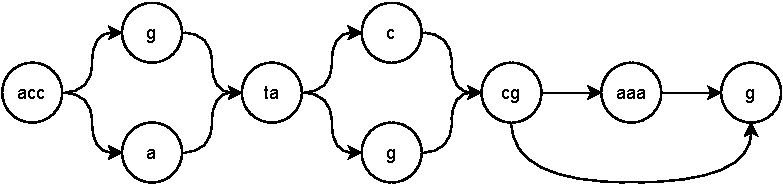
\includegraphics[width=\textwidth]{img/gra.pdf}
  \end{figure}
\end{esempio}
Studiando i cammini dei grafi ottengo tutte le rappresentazioni.\\
Questa rappresentazione però ha dei difetti, in quanto potrei avere cammini che
non rappresentano nessuna sequenza di partenza. Pensando all'esempio sopra
potrei avere il cammino in rosso che non rappresenta nessuna delle tre sequenze:
\begin{figure}[H]
  \centering
  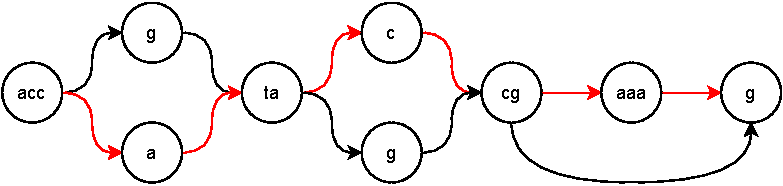
\includegraphics[width=\textwidth]{img/gra2.pdf}
\end{figure}
Rappresento quindi più di quello che voglio rappresentare.\\
Un pangenoma è un grafo che rappresenta una popolazione senza fare grandi
distinzioni, avendo percorsi che non sono riscontrabili in nessun individuo
della popolazione. Si ha comunque che il concetto di sequenza non è più
adeguato. Il grafo di una popolazione è enorme e comunque, tramite colori, si
possono distinguere i vari percorsi della popolazione (distinguendo facilmente
``tracce comuni''). Parlando quindi di \textbf{genoma di riferimento} o si parla
di quello specifico di un individuo o si parla del pangenoma di una popolazione,
con le varianti.\\
Dal punto di vista di \textit{file} le varianti vengono date in un file
\textbf{Variant Call Format (\textit{VCF})}. L'input classico dei software è
quindi spesso un VCF, così come l'output.
\section{Progetti attuali}
Vediamo ora quali sono i grandi progetti su larga scala attualmente in corso:
\begin{itemize}
  \item \textbf{The Cancer Genome Atlas Pan-Cancer Analysis Project
    (\textit{TCGA})}, che cerca di costruire un catalogo delle caratteristiche
  genomiche dei tumori, ovvero un catalogo delle mutazioni genomiche associate a
  tumori (ad esempio quello del seno si sa che è legato alla mutazione del gene
  BRCA che si sa bene dov'è)
  \item \textbf{The 1000 Genomes Project Consortium: A global reference for
    human genetic variation}, che cerca di ricostruire e raffinare un
  sequenziamento di diversi genomi per costruire 
  un genoma di riferimento per una popolazione, nel dettaglio umana, (in formato
  VCF) 
  \item \textbf{Trans-Omics for Precision Medicine}, il progetto per la medicina
  translazionale 
  \item \textbf{The Computational Pangenome Consortium}, che mira a studiare
  nuovi strumenti software che possano trattare il grafo del pangenoma visto che
  la maggioranza del software attuale ancora funziona su sequenze e non su grafi
\end{itemize}
\section{Sequenziamento del DNA}
Il sequenziamento (che letteralmente significa ``produrre la sequenza'')
solitamente si svolge concatenando diverse operazioni: 
\begin{enumerate}
  \item estrazione del DNA
  \item si ha una ``libreria preparatoria'' dove si mette del materiale genetico
  su un materiale preparatorio
  \item si ha un meccanismo di ``copie'' tramite PCR o simili
  \item si mettono i sample genomici in una macchina di sequenziamento che
  produce in output i dati
\end{enumerate}
Un genoma non può essere letto ``nucleotide per nucleotide'' e i biologi, con la
tecnologia attuale producono le cosiddette \textbf{read} del DNA originali. Si
hanno due tipi di read:
\begin{itemize}
  \item \textbf{read}, dette anche \textbf{short read}, lunghe circa 100
  basi. Illumina produce tendenzialmente 100 o al più 150 basi
  \item \textbf{long read}, lunghe circa 10000 basi (se non di più, anche 20000)
\end{itemize}
Per ottenere il sequenziamento si ha un processo in cui:
\begin{itemize}
  \item si divide il genoma in due parti, ``aprendo'' il filamento di DNA per
  permetterne la lettura
  \item si ha la \textbf{generazione delle read} da copie multiple del genoma
  tramite un processo biologico svolto dai macchinari, che sfruttano processi
  chimici 
  \item si ha poi \textbf{l'assemblaggio dei frammenti}, ovvero un processo
  computazionale dove tramite algoritmi si assemblano le varie read per ottenere
  il genoma di partenza, avendo che le read hanno pezzi in \textit{overlap}
\end{itemize}
Il problema del sequenziamento risale alla fine degli anni settanta con Sander e
Gilbert che avevano studiato un processo di replicazione dando le basi allo
studio del sequenziamento.\\
Dopo il sequenziamento dell'uomo si è passati a sequenziare molti altri
organismi.\\
Oggi il sequenziamento è reso semplice dalla tecnologia. Un esempio è la
tecnologia MinION, così piccola sta stare in una mano, che produce \textit{long
  read} (anche se comunque con diversi errori). MinION è una tecnologia di
\textit{Oxford Nanopore}. MinION è USB ed è fatta per
biologi che devono sequenziare in situazioni d'emergenza (esempio banale un
biologo in Africa in piena emergenza Ebola). L'elaborazione dati viene fatta da
un server.\\
Il primo sequenziamento è costato 3 miliardi di dollari per diversi anni, ora si
fa in meno di 40 ore a 5000 dollari. Di recente si è passati addirittura a poche
ore per un costo di circa 1000 dollari. Tornando alla \textit{legge di Moore} si
ha che il costo è collassato rispetto alla legge e quindi la capacità delle
tecnologie di sequenziamento è molto maggiore della capacità di processare i
dati, per quanto visto ad inizio capitolo. Si hanno quindi tanti dati ma non si
è in grado di elaborarli.\\
Si tratterà anche il \textbf{confronto di genomi} per studiare poi gli aspetti
evoluzionistici, tramite \textbf{alberi evolutivi}, anche \textbf{alberi
  evolutivi tumorali}. Il \textbf{confronto tra sequenze} 
permette di studiare le evoluzioni, anche quelle tumorali, dove si hanno
mutazioni radicali di DNA. Approfondiremo anche tali mutazioni e il loro effetto
(basta il cambio di una base per portare, ad esempio, all'anemia
falciforme). Studieremo quindi anche come fare gli\textbf{
  allineamenti}. Approfondiremo il discorso della \textbf{filogenesi} e della
\textbf{filogenesi tumorale}.\\
Tutto questo, in questo ultimo anno, è stato applicato allo studio di
\textbf{sars-cov-2}, avendo lo studio delle variazioni. \\
Verrà approfondito anche il discorso del \textbf{riarrangiamento}.
\chapter{Grafi di assemblaggio}
La prima tematica che affrontiamo è l'assemblaggio delle read tramite grafi. Per
questo problema abbiamo quindi:
\begin{itemize}
  \item \textbf{input}: collezioni di read (short read e/o long read)
  \item \textbf{output}: grafo di assemblaggio da cui estrarre un cammino o
  un'unica sequenza
\end{itemize}
Si hanno principalmente due tipi di grafo:
\begin{itemize}
  \item \textbf{grafo di De Brujin (\textit{DBG})} (\textit{si legge ``grafo di
    de broin''}), che si prestano più per \textit{short read} (da 100 o 150
  basi) 
  \item \textbf{grafo di overlap}, più comodo in caso di \textit{long read}
\end{itemize}
Si useranno per questi scopi varie nozioni, tra cui:
\begin{itemize}
  \item relazione di prefisso/suffisso tra k-mers
  \item relazione di prefisso/suffisso tra read
  \item Longest Common Prefix tra sequenze
  \item estrazione di cammino di Eulero dal grafo
  \item estrazione di cammino Hamiltoniano dal grafo
  \item Maximal Exact Matches (\textit{SMEMs})
  \item Burrows Wheeler Transform (\textit{BWT})
  \item indici succinti (come FM-Index)
  \item suffix tree e suffix array
  \item bloom filters, nati in ambito fisico e usati ora in ambito BigData
  \item min-hash e min-sketch, usati anche nelle reti neurali e nel Deep
  Learning quando si ha a che fare con grandi moli di dati
\end{itemize}
Studiare i grafi di assemblaggio può essere utile anche in ottica di applicare
procedimenti simili ad altri problemi posti dai biologi.
\section{Grafi in bioinformatica}
In bioinformatica infatti uno strumento molto usato, anche oltre il
sequenziamento, è quello dei \textbf{grafi}.\\
In letteratura la nozione di grafo compare nel 1735 con il \textbf{grafo di
  Eulero}, con Eulero che, si dice, fosse ossessionato dal problema dei
\textbf{ponti di K\"{o}nigsberg}, volendo trovare il ciclo che attraversasse
ogni ponte solo una volta. Ogni isola di K\"{o}nigsberg diventava un nodo e ogni
ponte tra isole un arco tra nodi. Da qui la definizione del problema.
\begin{definizione}
  Il  \textbf{problema del ciclo Euleriano} consiste nel trovare un ciclo in un
  grafo tale che visiti ogni arco una e una sola volta prima di tornare al punto
  di partenza. Si può passare dallo stesso nodo più volte.\\
  Questo problema si dimostra risolvibile in \textbf{tempo lineare} sull'input
  $G=(V,E)$. 
\end{definizione}
Vediamo poi il ``problema duale'', quello in cui si vuole fare un cilo che non
visiti due volte uno stesso nodo.
\begin{definizione}
  Il  \textbf{problema del ciclo Hamiltoniano} consiste nel trovare un ciclo in un
  grafo tale che visiti ogni vertice una e una sola volta prima di tornare al punto
  di partenza.\\
  Questo problema si dimostra essere \textbf{NP-complete}.
\end{definizione}
La differenza di complessità di questi due problemi sarà qualcosa che bisognerà
considerare parlando dello studio dei grafi in bioinformatica. Anche solo il
problema dell'assemblaggio si vedrà è riducibile alla visita di un grafo (quindi
non potremo formularlo come un problema di ciclo Hamiltoniano, la cui soluzione
potrebbe richiedere anni).\\
La comparsa dei grafi nel mondo chimico è intorno a metà del 1800 con Cayley che
li usò per rappresentare strutture chimiche, nel dettaglio usò \textbf{alberi}
(che ricordiamo esserei grafi connessi aciclici) per contare gli isomeri
strutturali.\\
In biologia l'uso dei grafi è stato introdotto a metà 1900 con l'esperimento di
Benzer, che capì l'importanza dei grafi mentre cercava di distinguere quando
determinati virus attaccano determinati batteri. Benzer è riuscito a mostrare che
il DNA di questi virus era \textit{lineare} mentre prima si congetturava che il
DNA avesse delle biforcazioni. Per capire che non avesse delle biforcazioni ha
sfruttato la capacità di alcuni geni dei virus di aggredire batteri,
rappresentando la cosa coi \textbf{grafi ad intervallo}.
\begin{definizione}
  Nella teoria dei grafi, un \textbf{grafo d'intervallo} è il grafo
  d'intersezione di un 
  multiinsieme di intervalli sulla linea reale. Ha un solo vertice per ciascun
  intervallo dell'insieme, e uno spigolo tra ogni coppia di vertici
  corrispondenti agli intervalli che
  intersecano.
  \footnote{\url{https://it.wikipedia.org/wiki/Grafo\_d\%27intervallo}}\\
  In poche parole associo una lettera ad ogni intervallo e collego nel grafo i
  vertici corrispondenti alla lettera qualora i due intervalli abbiano
  sovrapposizioni.
\end{definizione}
Il punto di svolta si ha però nel 1977 col sequenziamento e i due metodi di
Sanger (che è tutti gli effetti il primo metodo di sequenziamento) e Gilbert,
entrambi chimici. Entrambi i metodi generano frammenti etichettati di lunghezza
variabile che vengono ``letti'' tramite elettroforesi. \\
\textit{Non approfondiamo nel dettaglio i metodi, essendo prettamente chimici e
  biologici}.
\section{Superstringhe e grafo di overlap}
L'assemblaggio dei frammenti del DNA è invece un problema prettamente
computazionale, avendo l'assemblaggio dei singoli frammenti, ovvero delle
\textbf{read} prodotte dal sequenziamento, anche in più copie, in un'unica
sequenza genomica, detta \textbf{superstringa}. \textit{Fino alla fine degli
  anni '90 l'assemblaggio di frammenti del genoma umano era visto come un
  problema intrattabile.}
\begin{definizione}
  Definiamo \textbf{stringa} come la concatenazione di simboli di un alfabeto
  $\Sigma$.\\
  In bioinformatica spesso si ha $\Sigma=\{a,c,g,t\}$
\end{definizione}
\begin{definizione}
  Definiamo il \textbf{shortest superstring problem (SSP)} come la ricerca,
  dato un insieme di stringhe, di trovare la più corta superstringa che le
  contiene tutte. So hanno quindi:
  \begin{itemize}
    \item \textbf{input}: una collezione $s_1,s_2,\ldots,s_n$ di stringhe che
    possono anche essere lunghe uguali o a lunghezza variabile
    \item \textbf{output}: una stringa $s$ che contiene tutte le stringhe
    $s_1,s_2,\ldots,s_n$ dell'input come sottostringhe tale che $|s|$, ovvero la
    lunghezza della stringa $s$, sia \textbf{minima}
  \end{itemize}
  Questo problema è \textbf{NP-complete} e assume che non ci siano errori di
  sequenziamento nella produzione delle stringhe $s_1,s_2,\ldots,s_n$.\\
  \textbf{La shortest superstring potrebbe non essere unica}.
\end{definizione}
\begin{esempio}
  Vediamo un esempio di shortest superstring. Si assume per semplicità alfabeto
  binario $\Sigma=\{0,1\}$.\\
  Si ha la collezione di stringhe binarie in input (che nel dettaglio sono tutte
  le possibili combinazioni di 3 simboli binari):
  \[C_I=\{000,001,010,011,100,101,110,111\}\]
  Si può verificare che la shortest superstring è:
  \[s=0001110100\]
\end{esempio}
Con la shortest superstring ho letteralmente assemblato le stringhe in input.\\
Le read determinano la \textbf{coverage (\textit{copertura})} del DNA. Per
valutare il coverage vado a vedere ogni base da quante read è coperta. Con
Illumina ho un coverage di almeno 50x, quindi ogni posizione è coperta da almeno
50 read (lunghe ciascuna $\sim$150 basi). Per poter ricostruire la sequenza di
DNA originale serve una certa quantità di coverage. Una coverage bassa potrebbe
impedire la ricostruzione. Illumina va dal 50x minimo anche a 80x.
MinION, della Oxford Nanopore, produce long read anche di 20000 basi ma con
basso coverage, anche 3x, ma avendo read lunghe si riesce comunque ad
assemblare. Quindi se ho long read mi basta un basso coverage mentre se ho short
read mi serve un elevato coverage, avendo un insieme di read molto ``fitto'' e
con poca ``sparsità'', in quanto si avrebbero gap, con zone non coperte. Il
coverage è comunque dato ``per media'' e quindi poter comunque avere buchi.\\
Il punto chiave che mi permette di ricostruire il DNA è la sovrapposizione tra
le varie read. Il DNA inoltre ha ripetizioni e questo costituisce, purtroppo, un
limite all'assemblaggio e in merito studieremo il \textbf{fragment assembly
  problem}, che serve anche in altri contesti, oltre a quello dell'assemblaggio
del DNA. Fin'ora abbiamo anche trascurato anche un altro problema, gli
\textbf{errori di sequenziamento}, dati dal fatto che il processo di sequenziare
non è \textit{ottimo}, ovvero privo di errori, dove con errore si intende che
nel DNA si ha una certa base e nella read prodotta dal sequenziamento se ne ha
un'altra. In fase di assemblaggio questo tipo di errore comporta che non si
riesce a sovrapporre bene le read, non potendo vedere più alcuni
\textbf{overlap} tra coppie read. Si ha quindi \textbf{perdita di informazione
  dell'overlap} e diventa più complicato assemblare il DNA, non impossibile ma
più complicato.
\begin{esempio}
  Si hanno un pezzo di DNA e tre read che sono sovrapponibili:
  \begin{table}[H]
    \centering
    \begin{tabular}{cccccccccc}
      \hline
      & 1 & 2 & 3 & 4 & 5 &6 &7 &8\\
      \hline
      $DNA=$ & a & c & c & g & t &a &c &g\\
      \hline
      $R_1=$ & a & c & c & g & t &&&\\
      $R_2=$ &  & c & c & g & t & a &&\\
      $R_3=$ &  &  &  & g &t & a &c & g&\\
    \end{tabular}
  \end{table}
  Possiamo quindi assemblare il pezzo di DNA.\\
  Ma se ipotizziamo di avere un errore di sequenziamento con la terza base della
  seconda read:
   \begin{table}[H]
    \centering
    \begin{tabular}{cccccccccc}
      \hline
      & 1 & 2 & 3 & 4 & 5 &6 &7 &8\\
      \hline
      $DNA=$ & a & c & c & g & t &a &c &g\\
      \hline
      $R_1=$ & a & c & c & g & t &&&\\
      $R_2=$ &  & c & c & \textbf{c} & t & a &&\\
      $R_3=$ &  &  &  & g &t & a &c & g&\\
    \end{tabular}
  \end{table}
  Diventa più difficile assemblare.
\end{esempio}
Il tasso di errore nei macchinari Illumina è dello 0.01\%, avendo circa due
errori per read lunga 150. Per MinION si ha un tasso d'errore anche di circa il
10\%, quindi ogni 50 basi ho una serie d'errore. Di recente, in ambito long
read, si stanno progettando i \textbf{PacBio HiFi} (con HiFi che qui sta per
``high quality framents'') che producono long read con tasso d'errore allo
0.1\%, facendo ben sperare per il futuro.\\
Tra i primi informatici che hanno fatto sequenziamento abbiamo Gene Myers che
era un esperto di algoritmi su stringhe e di pattern matching (parte attiva
nella creazione dei suffix array), nonché responsabile della creazione
dell'algoritmo di assemblaggio (famoso anche per BLAST). Gene Myers era un
esperto del problema della shortest superstring. A partire dalla tecnica di
costruzione della shortest superstring ha sviluppato l'algoritmo di
assemblaggio. Vediamo quindi, in primis, come costruire la shortest
superstring. Per farlo bisogna in primis capire come confrontare le varie
stringhe in input e come ``foldarle''. Per farlo faccio l'overlap che però a
questo punto necessita di una definizione formale.
\begin{definizione}
  Definiamo \textbf{overlap} tra una coppia di stringhe $s_i$ e $s_j$ in input
  come il più lungo prefisso di $s_j$ che ha un match perfetto (coincide) con un
  suffisso di $s_i$. Posso anche dire che è il più lungo suffisso di $s_i$ che
  ha un match perfetto con un prefisso di $s_j$, ribaltare la definizione non
  cambia. L'overlap tra le due stringhe si indica con: 
  \[ov(s_i,s_j)\]
  Ricordiamo che una stringa la posso scrivere in modo scomposto in due modi:
  \begin{itemize}
    \item $s_i=s_i'x$, con $x$ suffisso
    \item $s_j=xs_j'$, con $x$ prefisso
  \end{itemize}
  Tendenzialmente si prende l'\textbf{overlap più lungo}.
\end{definizione}
\begin{esempio}
  Siano:
  \[s_i=accgtgtgt\]
  \[s_j=gtgtgtccaa\]
  Allora si ha che:
  \[ov(s_i,s_j)=gtgtgt\]
  con l'overlap lungo 6.
\end{esempio}
Proseguiamo quindi con il calcolo della shortest superstring dopo aver calcolato
l'overlap di tutte le stringhe in input.\\
Creo un grafo con un nodo per ogni sequenza, etichettato con la sequenza
stessa. Tracciamo quindi un arco tra due nodi sse i due nodi sono in overlap,
associando all'arco la lunghezza dell'overlap.\\
Una tecnica per fare il grafo consiste in:
\begin{itemize}
  \item collegare a priori di tutti i nodi ottenendo un grafo completo non
  orientato 
  \item per ogni coppia di stringhe $s_i$ e $s_j$ metto l'arco pesato con
  l'overlap massimo $ov(s_i,s_j)$, dando anche direzione all'arco. Eventualmente
  posso anche dare doppio peso all'arco in base alla direzione. Si è ottenuto il
  \textbf{grafo di overlap}, che quindi è un grafo orientato (se in entrambi i
  versi non ho overlap lo lascio per praticità senza orientamento con peso 0)
\end{itemize}
\begin{esempio}
  Sia la collezione di stringhe in input:
  \[C_i=\{atc,cca,cag,tcc,agt\}\]
  e costruisco il grafo completo come detto sopra:
  \begin{figure}[H]
    \centering
    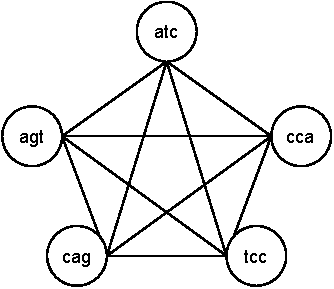
\includegraphics[scale = 0.9]{img/gra3.pdf}
  \end{figure}
  Aggiungo quindi i pesi relativi agli overlap dando l'eventuale orientamento e
  ottengo il grafo di overlap:
  \begin{figure}[H]
    \centering
    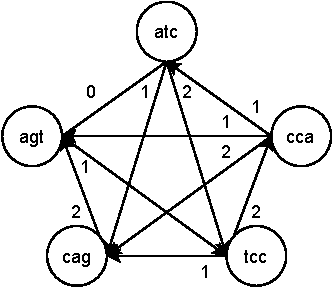
\includegraphics[scale = 0.9]{img/gra4.pdf}
  \end{figure}
\end{esempio}
Per calcolare la shortest superstring dovremo calcolare un certo cammino sul
grafo di overlap. Sicuramente un cammino che visita tutti i nodi mi porta ad
avere una superstringa. Vediamo quindi una prima idea intuitiva:
\begin{esempio}
  Riprendendo il grafo di overlap dell'esempio precedente faccio:
  \begin{itemize}
    \item parto dal nodo $atc$ e lo aggiungo alla superstringa, che per ora è
    $s=atc$ 
    \item seguo l'arco di peso 2 e arrivo in $tcc$
    \item aggiungo $c$ (ovvero la parte non in overlap) alla superstringa, che
    per ora è $s=atcc$ 
    \item seguo l'arco di peso 2 e arrivo in $cca$
    \item aggiungo $a$ (ovvero la parte non in overlap) alla superstringa, che
    per ora è $s=atcca$
    \item seguo l'arco di peso 2 e arrivo in $cag$
    \item aggiungo $g$ (ovvero la parte non in overlap) alla superstringa, che
    per ora è $s=atccag$
    \item seguo l'arco di peso 2 e arrivo in $agt$
    \item aggiungo $t$ (ovvero la parte non in overlap) alla superstringa, che
    per ora è $s=atccagt$ 
    \item mi fermo avendo visitato tutti i nodi
  \end{itemize}
  Alla fine ho:
  \[s=atccagt\]
  che so essere una superstringa.
\end{esempio}
Si vede che il cammino, a conferma, tocca ogni vertice una e una sola volta,
avendo un cammino Hamiltoniano ma, avendo i pesi, abbiamo a che fare con un
\textbf{Traveling Salesman Problem (\textit{TSP})}. Dobbiamo però dimostrare che
la superstringa ottenuta è anche la più breve. \\
Diamo però una piccola definizione formale del grafo di overlap.
\begin{definizione}
  Definiamo il \textbf{grafo di overlap} $G_{ov}=(V,E)$ tale che, data una
  collezione di stringhe $s_1,\ldots,s_n$:
  \begin{itemize}
    \item $V=\{s_1,\ldots,s_n\}$
    \item $E$ è definito in modo che ogni arco $(s_i,s_j)\in E$ è un arco
    orientato da $s_i$ a $s_j$ di peso $|ov(s_i,s_j)|$ (quindi pesato con la
    lunghezza dell'overlap)
  \end{itemize}
\end{definizione}
Si dimostra poi che il \textbf{cammino Hamiltoniano di massimo costo}
``produce'' una shortest superstring. Facciamo una dimostrazione non
formale. Innanzitutto per ``produce'' si intende che, dato il cammino prodotto
da Hamilton di massimo costo, con i vertici etichettati dalle stringhe
$s_{i,1},s_{i,2},\ldots,s_{i,n}$, la superstringa si ottiene sapendo che una
stringa $s_{i,j+1}$ che è ha un prefisso in overlap con al precedente stringa
$s_{i,j}$ la si può scrivere come: 
\[s_{i,j+1}=ov(s_{i,j},s_{i,j+1})\cdot x_{i,j+1}\]
Possiamo anche dire che:
\[r(s_{i,j},s_{i,j+1})=x_{i,j+1}\]
indicando con $x_{i,j+1}$ la parte della stringa fuori dall'overlap, il
``resto'' possiamo dire. A questo
punto so che la superstringa parte con $s_{i,1}$ e prosegue concatenando i vari
$x_{i,j+1}$:
\[s=s_{i,1}\cdot x_{i,2}\cdot x_{i,3}\cdot\ldots\cdot \cdot x_{i,n}\]

Bisogna dimostrare che il cammino Hamiltoniano di massimo peso coincide con la
shortest superstring. Bisogna dimostrare che:
\begin{itemize}
  \item un cammino Hamiltoniano di massimo peso calcolato come sopra è una
  superstringa, e questo di dimostra perché tocca ogni vertice e quindi ogni
  stringa che di conseguenza viene inclusa
  \item la superstringa appena calcolata è la più breve e per dimostrarlo si ha
  l'intuizione che se massimizzo l'overlap ``globale'' minimizzo la lunghezza
  della superstringa 
\end{itemize}
\begin{figure}
  \centering
  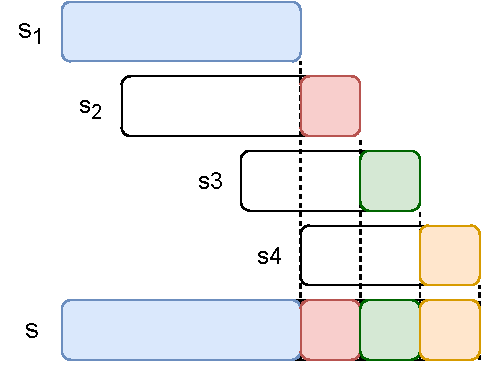
\includegraphics[scale = 0.8]{img/ssp.pdf}
  \caption{Esempio di formazione di una shortest superstring a partire da una
    collezione di stringhe sfruttando i ``resti'' degli overlap}
\end{figure}
Il calcolo della shortest superstring può quindi risolvere l'assemblaggio di
stringhe anche se \textbf{si ricorda che il problema del cammino Hamiltoniano è
  NP-complete}. \\
La miriade di read però, quando ci lavorò per primo Gene Myers, rendeva
davvero difficile il calcolo (problema NP-complete e hardware storicamente poco
potente). Servirono quindi anni per il primo calcolo, circa una quindicina,
usando appunto il metodo della superstringa.\\
Si ha però un'euristica per calcolare la superstringa, usando un
\textbf{algoritmo 2-approssimante} usando la \textbf{tecnica greedy}. In base a
questa tecnica si sceglie sempre l'arco che pesa di più nel senso che ordino in
ordine di peso tutti gli archi e faccio gli overlap tra le stringhe.
%1.24.30 lezione 2

Non si ha la
soluzione ottima ma appunto è 2-approssimante.
\end{document}  
% LocalWords:  clock burst bioinformatico bioinformatici aplotipi VCF NP
% LocalWords:  sottostringhe dell'overlap shortest superstring L'overlap
% LocalWords:  superstringa
